% 
% Annual Cognitive Science Conference
% Sample LaTeX Paper -- Proceedings Format
% 

% Original : Ashwin Ram (ashwin@cc.gatech.edu)       04/01/1994
% Modified : Johanna Moore (jmoore@cs.pitt.edu)      03/17/1995
% Modified : David Noelle (noelle@ucsd.edu)          03/15/1996
% Modified : Pat Langley (langley@cs.stanford.edu)   01/26/1997
% Latex2e corrections by Ramin Charles Nakisa        01/28/1997 
% Modified : Tina Eliassi-Rad (eliassi@cs.wisc.edu)  01/31/1998
% Modified : Trisha Yannuzzi (trisha@ircs.upenn.edu) 12/28/1999 (in process)
% Modified : Mary Ellen Foster (M.E.Foster@ed.ac.uk) 12/11/2000
% Modified : Ken Forbus                              01/23/2004
% Modified : Eli M. Silk (esilk@pitt.edu)            05/24/2005
% Modified : Niels Taatgen (taatgen@cmu.edu)         10/24/2006
% Modified : David Noelle (dnoelle@ucmerced.edu)     11/19/2014

%% Change "letterpaper" in the following line to "a4paper" if you must.

\documentclass[10pt,letterpaper]{article}

\usepackage{hyperref}
\usepackage{cogsci}
\usepackage{pslatex}
\usepackage{amsfonts}
\usepackage{graphicx}
\usepackage{apacite}
\usepackage{color}
\usepackage{todonotes}

\definecolor{Red}{RGB}{255,0,0}
\newcommand{\red}[1]{\textcolor{Red}{#1}}

\newcommand{\jd}[1]{\green{$^*$}\marginpar{\footnotesize{JD: \green{#1}}}}

\newcommand{\subsubsubsection}[1]{{\em #1}}
\newcommand{\eref}[1]{(\ref{#1})}
\newcommand{\tableref}[1]{Table \ref{#1}}
\newcommand{\figref}[1]{Figure \ref{#1}}
\newcommand{\appref}[1]{Appendix \ref{#1}}
\newcommand{\sectionref}[1]{Section \ref{#1}}

\title{Why do you ask? To be informative.}
 
\author{{\large \bf Robert X.~D.~Hawkins (rxdh@stanford.edu)} \AND {\large \bf Andreas Stuhlm\"uller (andreas@stuhlmueller.org)}\\ 
	\AND
	{\large \bf Judith Degen (jdegen@stanford.edu)} 
  \AND {\large \bf Noah D.~Goodman (ngoodman@stanford.edu)} \\
  Department of Psychology, 450 Serra Mall \\
  Stanford, CA 94305 USA}


\begin{document}

\maketitle


\begin{abstract}


\textbf{Keywords:} 
questions; answers; computational pragmatics; theory of mind; 
\end{abstract}

\section{Introduction}
\label{sec:intro}

Suppose your friend approaches you and asks, ``Who is coming to the concert tonight?'' How do you respond? You certainly don't need to give the full list of attendees -- most of whom you do not know -- even though they would all technically be valid answers. Instead, you might only mention the set of \emph{mutual acquaintances} you know are planning to come, assuming that your friend doesn't care about the rest of the crowd. Now, imagine a different scenario. Suppose that you're waiting in line at the box office and want to find out whether your acquaintances had tickets as well. What question would you ask to the person in the ticket booth? If you asked, ``Who is coming to the concert tonight?''  you would likely get a quizzical look and an answer like ``I don't know, a lot of people, why?'' Instead, you might have to directly ask about your friends. 

Since both questioners and answerers are so acutely sensitive to one another's intentions and knowledge, what makes a question useful? What makes an answer to a question useful? In this paper, we present three progressively more sophisticated computational models of question and answer behavior, which formalize and probe this deep interaction between the way answerers infer intentions and the way questioners signal them. We compare these models on the basis of two experiments in which participants must ask and answer questions given a fixed set of goals. We find that a sophisticated pragmatic answerer is needed to account for the data, and close by proposing that the purpose of questions in dialogue is to provide cues to the answerer about the questioner's goals and intentions.

A number of studies in psycholinguistics have provided evidence that answerers are both sensitive to a questioner's goals and attempt to be informative with respect to those goals. For example, when people are asked `Do you have the time?'' they typically round their answers to the nearest 5 or 10 minute interval, even when they're wearing a digital watch \cite{DerHenstCarlesSperber02_RelevanceTellingTime}. However, if the question is preceded by the statement ``My watch stopped,'' people make their response precise to the minute  \cite{GibbsBryant08_OptimalRelevance}.

Similar evidence comes from a classic study where researchers called liquor merchants and asked, ``Does a fifth of Jim Beam cost more than \$5?'' If this was preceded by the statement, "I want to buy some bourbon,'' merchants gave the actual price significantly more frequently than when it was preceded by the statement, ``I've got \$5 to spend.'' In the former case, the merchant inferred that the questioner's goal was just to buy whiskey, so the exact price is the maximally relevant response. In the latter case, the merchant inferred that the questioner's goal was literally to find out whether or not they could afford the whiskey, hence a simple `yes'  sufficed \cite{Clark79_IndirectSpeechActs}. Context and questioner goals have also been implicated in accounts of identification questions like ``who is X?'' \cite{BoerLycan75_KnowingWho}, and to questions like ``where are you?'' that permit answers at many levels of abstraction \cite{Potts12_CardsDialogueCorpus}.

Recent formal models of pragmatics have made progress by incorporating speaker goals and a notion of informativeness with respect to these goals. However, these efforts have made the question itself somewhat redundant. If the answerer is so adept at using context to determine the relevant information, why does the questioner need to ask a question in the first place? Is it just a formality, to prompt the other for their information, or does it serve as a signal in itself? We claim that people ask questions in order to get useful answers. Thus, in order to predict the kinds of answers a given question will produce, the questioner must reason about the behavior of an answerer. This answerer does \emph{not} know the questioner's intentions  \emph{a priori} and instead must infer them using the question itself as a signal. Combined with the psycholinguistic data above, this model seeks to place question and answer behavior in the larger class of social behavior governed by theory of mind.

The rest of this paper is structured as follows. First, we specify a family of questioner and answerer agents extending the Rational Speech Act (RSA) framework \cite{frank2012, GoodmanStuhlmuller13_KnowledgeImplicature}, highlighting some points of divergence from previous RSA models. We then individuate three particular models in this family, representing progressively more sophisticated hypotheses about how questioners and answerers reason about their task. In particular, we compare a pragmatic answerer making inferences about the questioner's goals to two simpler models: one that takes into account only that an answerer wants to be maximally informative with respect to the explicit question asked (without inferring the questioner's underlying decision problem) and one that provides a literal answer to the question (without attempting to be maximally informative).  To compare these models, we derive predictions for a pair of experiments using a novel guessing-game task, and compare these predictions to human performance. In one phase of the task, we require participants to ask a question (from a fixed set of possible questions), given a decision problem. In the second phase, we require participants to give an answer (from a fixed set of possible answers) to a question (from a fixed set of possible questions). 

\section{A Rational Speech Act model of question and answer behavior}
\label{sec:model}

Suppose there is a set of distinct world states $\mathcal{W}$, a set of possible goals $\mathcal{G}$, a set of possible questions $\mathcal{Q}$, and a set of possible answers $\mathcal{A}$. These sets are all taken to be in common ground. We begin by thinking about how an optimal questioner should choose a question. Critically, instead of trying to impart information about the state of the world, a questioner attempts to \emph{learn information about a private goal}, sometimes called a QUD (or question under discussion) \cite{Roberts96_InformationStructureDiscourse}. A goal $g \in \mathcal{G}$ is a function that transforms a complete world state to a particular feature or features of that world that the questioner cares about, thus serving as a utility function on the distribution of worlds consistent with the answer. In order to learn information about their private goal $g$, the questioner reasons about how an internal model of an answerer would respond given some true world. 

\begin{itemize}

\item The \textbf{questioner} takes a goal $g \in \mathcal{G}$ as input and returns a distribution over questions $\mathcal{Q}$. It first computes a prior $P_g(w)$ over the features of the world relevant to their goal. For each question $q \in \mathcal{Q}$, it computes the expected information gain, averaged over all possible true worlds, and all possible responses the answerer could give. Information gain is measured as the  Kullback-Leibler divergence between the prior distribution $P_g(w)$ and the posterior distribution over world states after hearing the answerer's (hypothetical) response: $$P(q | g) \propto \sum_{a \in \mathcal{A}} \sum_{w^* \in \mathcal{W}} P(w^*) P(a | q, w^*) D_{KL}(P_g(w)\, \| \, P_g(w | q, a))$$ where $P(a | q,w^*)$ is the response distribution returned by reasoning about what an answerer would say in true world $w^*$ after hearing questioner $q$. Note that $P(g(w) | q, a)$ is just an `interpreter' function that gives the likelihood of different worlds given different question and answer pairs.

\end{itemize}

This questioner depends critically on the answer distribution $P(a | q, w^*)$, which will upweight questions that elicit useful answers and downweight questions that elicit vague answers. We now propose several different answerer agents that embody different assumptions about this distribution.

\begin{itemize}

\item The \textbf{literal answerer} takes a question utterance $q \in \mathcal{Q}$ and a true world state $w \in \mathcal{W}$ as input and returns a distribution over the answer space $\mathcal{A}$. It samples an answer  $a$ from $\mathcal{A}$ with prior probability $P(a)$ and conditions on the likelihood of the questioner inferring the true world $w$ from this answer, using only the interpreter function as a cue. Note that this agent ignores the question; it's only concern is to convey the true state of the world. This makes it equivalent to the speaker in previous RSA models.
$$P(a | q,w^*) \propto P(w = w^* | q, a) P(a) $$
\item The \textbf{explicit answerer} samples an answer  $a$ from $\mathcal{A}$ with prior probability $P(a)$, then uses the explicit utterance $q$ as a QUD when evaluating the likelihood of a world under an interpreter. 
$$P(a | q, w^*) \propto P_q(w= w^* | q, a) P(a)$$
\item The \textbf{pragmatic answerer} uses the questioner defined above as a generative model of questions given goals in order to estimate the likelihood of different goals given the question $q$. It samples an answer $a$ from $\mathcal{A}$ with prior probability $P(a)$, uses an internal model of the questioner to estimate the likelihood of different goals $g \in \mathcal{G}$ given their question $q$, and attempts to be informative with respect to this goal:
$$\begin{array}{rcl}
P(a | q, w^*) & \propto & P(g | q)  \times P_g(w = w^* | q, a) \times P(a)\\
                    & \propto & P(q | g)P(g) \times P_g(w = w^* | q, a)  \times P(a)\\
\end{array}$$
\end{itemize}

Finally, we must define the interpreter function that all of these agents are using to compute the likelihood of a world given a question and an answer. This is where all semantic assumptions about the meaning of a question and answer are contained. For the purposes of this paper, we will use the standard Groenendijk \& Stokhof semantics \citeyear{GroenendijkStokhof84_SemanticsOfQuestions}, where a question induces a partition $\mathcal{P}_q$ over the space of possible worlds, where each cell is an equivalence class corresponding to a different answer. An answer, then, selects a cell of this partition, denoted by $\mathcal{P}_q(a)$, which is a set.

\begin{itemize}
\item The \textbf{interpreter} takes a question $q$ and an answer $a$ and returns a distribution of worlds that are consistent with this pair:

$$P(w | q, a) = P(w) \mathbb{I}_{\mathcal{P}_q(a)}(w)$$

where $\mathbb{I}_A(w)$ is the indicator function returning 1 if $w \in A$ and 0 otherwise.
\end{itemize}
This concludes our specification of the model space. Within this computational framework, different theories of question and answer behavior can be formalized and compared on the basis of their predictions. Assumptions about what is held in common ground are made transparent, and we can systematically manipulate individual elements of the model to test how they affect overall predictions. Because these are probabilistic models, we can succinctly write them down and evaluate their predictions in a probabilistic programming language \cite{Goodman13_POPL}. The model predictions shown throughout the rest of the paper were computed using a language called WebPPL \cite{GoodmanStuhlmuller14_DIPPL}. Note that this specification diverges from previous work in the RSA framework in a few key ways: (1) for the questioner, we replace the goal of imparting information with the goal of learning information about the specified QUD and (2) \dots \todo[inline]{RDH: any other major differences?}

\begin{figure}
\begin{center}
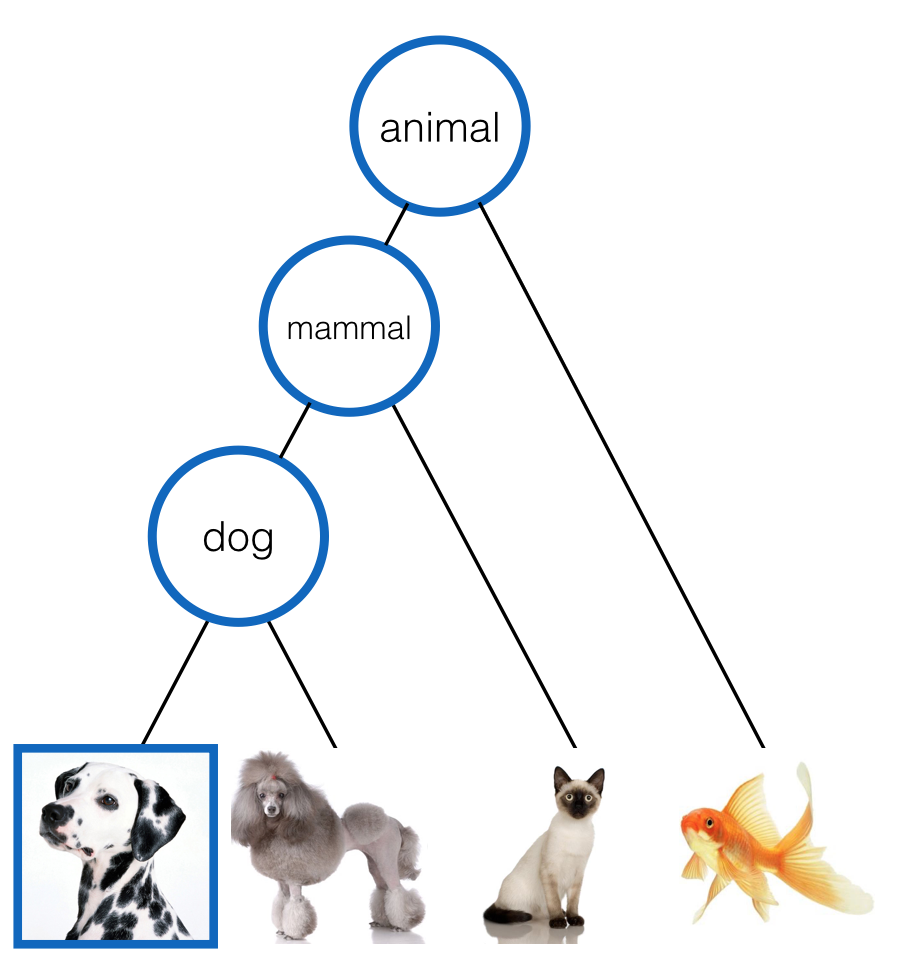
\includegraphics[scale = .2]{taskhierarchy}
\end{center}
\caption{Hierarchy of objects used in experiment 1}
\label{fig:taskhierarchy}
\end{figure}

\section{Experiment 1: \\ Questions and answers in a hierarchical world}

In order to test how questioners choose questions when given a decision problem, and how answerers choose answers under uncertainty about this decision problem, we designed a guessing-game task played by two players: a guesser and a helper. In this game, $4$ animals (a dalmatian, a poodle, a siamese cat, and a goldfish) were hidden behind $4$ gates. Note that these animals were arranged in a class hierarchy (see Fig. \ref{fig:taskhierarchy}). The guesser was given a private goal of finding one of the objects, and the helper had privileged information about the exact locations of each object. Before choosing a gate, the guesser could ask the helper a single question, and the helper could respond to this question by revealing the object behind a single gate. 

In terms of our model specification, the world space $\mathcal{W}$ is the set of $4! = 24$ possible assignments of four objects to four gates and the goal space $\mathcal{G}$ is the set of four objects that the guesser could possibly be trying to find, and the answer space $\mathcal{A}$ is the set of four gates that the helper could possibly reveal. The key constraint in the task, however, is that the guesser must choose from a \emph{restricted set of questions}: they may be trying to find the goldfish, but cannot directly ask `where is the goldfish?' Instead, the question space $\mathcal{Q}$ is the set of highlighted nodes in the hierarchy, including higher order nodes that are consistent with multiple answers. \todo[inline]{RDH: Need to define meaning functions for the interpreter, and actually highlight the nodes in the tree...}
\begin{figure*}[t!]
\begin{center}
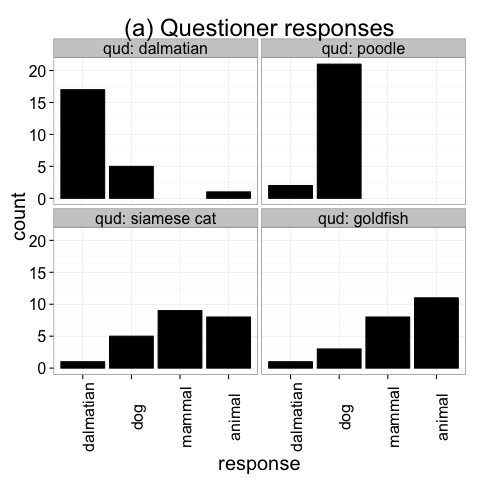
\includegraphics[scale = .5]{exp3_q}
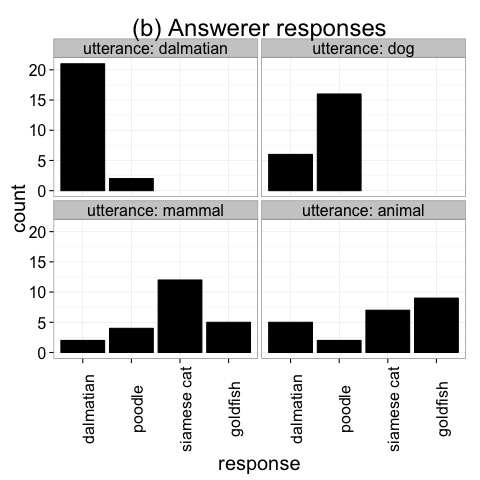
\includegraphics[scale = .5]{exp3_ans}
\end{center}
\caption{Experiment 1 results}
\label{fig:exp1res}
\end{figure*}
%\label{sec:expq}

We recruited 25 participants from Amazon Mechanical Turk to participate in this task. Each participant provided responses for four trials in the role of the questioner (corresponding to each goal in $\mathcal{G}$), and four trials in the role of the answerer (corresponding to each question in $\mathcal{Q}$). In order to collect responses for all elements of $\mathcal{G}$ and $\mathcal{Q}$, The order of� the questioner and answerer blocks was randomly assigned, and the order of stimuli within these blocks was also randomized\footnote{All materials are available on \href{https://github.com/hawkrobe/Q\_and\_A/tree/master/experiment3/versions/experiment3\_short}{Github}}. Two participants were excluded due to self-reported confusion about the task.

Results for the guesser role are shown in Figure \ref{fig:exp1res}(a). There are two primary trends to note in these data. First, questioners tend to choose the indirect question node closest to their goal when the direct question is unavailable. It is unsurprising that they ask about the `dalmatian` when looking for the dalmatian, but interesting that they strongly prefer asking about a `dog' when looking for the poodle, about a `mammal' when looking for the cat, and so on. \todo[inline]{RDH: need to statistically test whether this bar is really bigger than the others, which means I need to rerun the experiment for more power.} 


Results for the helper role are shown in Figure \ref{fig:exp1res}(b). The most striking feature of these data is how closely the answerer distribution matches the questioner distribution \todo[inline]{RDH: Possibly just because people did both... It might be the second-timers driving the effect, so we should separate out the different orders, or run it again between-subjects}. If the helper is asked about a `dog`, the dalmatian and poodle would be equally good literal answers to this question, but they strongly prefer to give the location of the poodle. Similarly, the dalmatian, poodle, and siamese cat are all mammals, but helpers prefer to respond to the `mammal' question by revealing the location of the cat. 

We now compare these results to the predictions of our family of models. At the very simplest level, our \emph{literal answerer} yields a uniform distribution over the four answers that are the case in the given world. This has important consequences for the corresponding questioner model: when this questioner reasons about which question would generate the most helpful answer from the literal answerer, they find no difference across questioners, and therefore have no preference over which question to ask. This is clearly not the case and we will not consider these options further.

At a slightly higher level of sophistication, we have an \emph{explicit answerer}. It up-weights answers that result in a distribution of worlds where as many as possible of the leaf nodes picked out by the question are in the correct location. Similarly, it down-weights answers that would mislead the questioner into the thinking that the leaf nodes mentioned in the question are in the wrong locations.  This model produces the answerer predictions depicted in Figure \ref{fig:exp1pred}(b), which successfully down-weights the least relevant alternatives but cannot break the symmetries between the explicitly relevant ones, and is therefore unable to satisfactorily account for our data. \todo[inline]{RDH: need to make the scatter plot for this `bad' model to show how much worse it is...}

While our `explicit answerer' model cannot account for answerer data, it does provide a foundation for a reasonably well-performing questioner model. When the questioner selects questions that maximize the expected information gain of the explicit answerer's response, it produces the distribution of questions shown in Figure \ref{fig:exp1pred}(a) \dots \todo[inline]{RDH: Need to discuss how we fit the rationality parameters somewhere }

Finally, we examine a pragmatic answerer that begins by estimating the likelihood of the questioner having a goal $g$ given the question being asked. It then applies this distribution of goals as the criterion for whether an answer is useful: it prefers answers for which the distribution of consistent worlds have the item specified by the particular goal is in the right position. The results for this answerer are depicted in Figure \ref{fig:exp1pred}(c).

To address concerns that the preceding results were due to particular features of the design such as the one-to-one mapping from goals to questions and from questions to answers, which gives the task the sense of an 'elimination game,' we ran a second experiment using a larger hierarchy \dots

\section{Experiment 2: }
\label{sec:expa}

\red{XXX TODO}

\begin{figure*}[t!]
\begin{center}
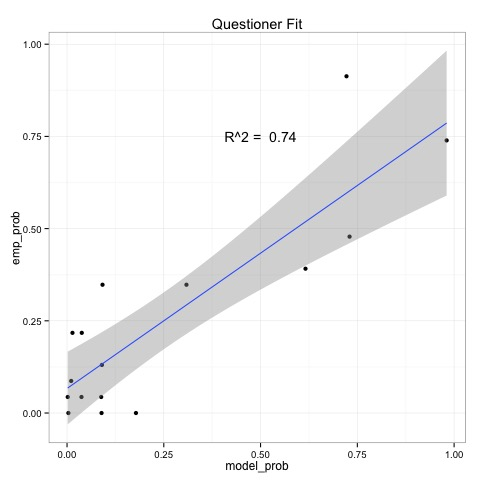
\includegraphics[scale = .33]{bestQuestioner}
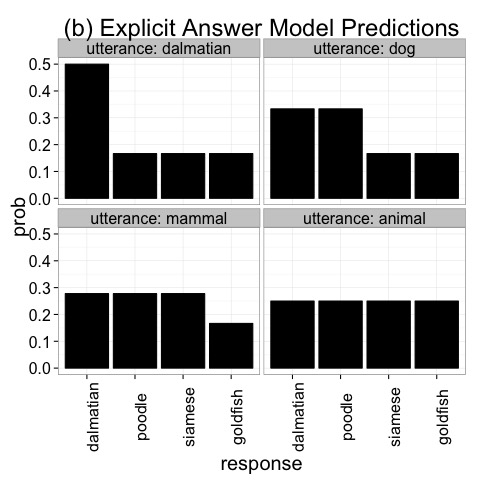
\includegraphics[scale = .33]{Exp3ExplicitAnswerPrediction}
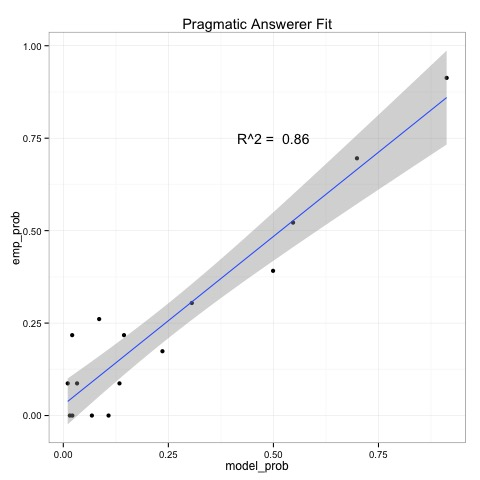
\includegraphics[scale = .33]{bestPragAnswerer}
\end{center}
\caption{Experiment 1 model predictions \todo[inline]{RDH: Need to replace the center plot with a scatter plot, and also include the `pragmatic questioner' }}
\label{fig:exp1pred}
\end{figure*}

\section{Related work}

Our account of question and answer behavior ultimately converges on a similar solution as contemporary decision theoretic or game theoretic accounts in linguistics. These theories were a response to early work on question and answer semantics, which focused on the notion of informativeness. In Groenendijk \& Stokhof's \citeyear{GroenendijkStokhof84_SemanticsOfQuestions} theory of question and answer semantics, asking a question induces a partition over the space of possible worlds, where each cell of the partition corresponds to a possible answer. An answer, then, consists of eliminating cells in this partition, and the most useful answers are those that eliminate all relevant alternatives to the true world. However, as van Rooy \cite{VanRooy03_QuestioningDecisionProblems} and others \cite{Ginzburg95_ResolvingQuestions} have pointed out, this predicts that \emph{wh}-questions like ``Where can I buy an Italian newspaper?'' can only be fully resolved by exhaustively mentioning whether or not such a newspaper can be bought at each possible location. Clearly, this is not the case: a single nearby location would suffice. These theories also cannot account for other contextual variation in what counts as a useful answer, such as questions like ``where are you?'' 

More recent theories have tried to fix these problems by introducing some consideration of the questioner's goals. van Rooy \citeyear{VanRooy03_QuestioningDecisionProblems}, for instance, formalizes these goals as a decision problem faced by the questioner. A useful answer under this decision theoretic account is one that maximizes the expected value of the questioner's decision problem. A useful question is one that induces a sufficiently fine-grained partition, optimally distinguishing the worlds relevant to the decision problem. While this framework elegantly accounts for the context-dependence and relevance-maximization of question and answer behavior, it assumes that the questioner's decision problem is known \emph{a priori} by the answerer. If this were the case, the act of asking questions would seem irrelevant: why wouldn't the answerer directly tell the questioner which action to take? 

\section{General discussion}
\label{sec:gd}

Humans are experts at inferring the intentions of other agents from their actions \cite{TomaselloCarpenter___Moll05_IntentionsCulturalCognition}. Given simple motion cues, for example, we are able to reliably discern high-level goals such as chasing, fighting, courting, or playing \cite{BarrettToddMillerBlythe05_IntentionFromMotionCues, HeiderSimmel44_ApparentBehavior}. Experiments in psycholinguistics have shown that this expertise extends to speech acts as well.  Behind every question lies some goal or intention. This could be an intention to obtain an explicit piece of information (``Where can I get a newspaper?''), signal some common ground (``Did you see the game last night?''), test the answerer's knowledge (``If I add these numbers together, what do I get?''), politely request the audience to take some action (``Could you pass the salt?''), or just to make open-ended small talk (``How was your weekend?''). These wildly different intentions seem to warrant different kinds of answers, even if the explicit question is expressed using the same words.

In this paper we have presented computational-level evidence that answerer behavior is best described by a pragmatic model that reasons about questioner intentions, using the question utterance as a signal. This analysis provides a novel perspective on the role of questions in dialogues: it is well-accepted under the Gricean view that answerers strive to be relevant, but we find that there is also a burden placed on the questioner to provide sufficient information about should be considered relevant in the first place. By artificially restricting the question space in our experiments, we have shown that when necessary, questioners can reliably choose an optimally informative signal.

\red{XXX}

\bibliographystyle{apacite}

\setlength{\bibleftmargin}{.125in}
\setlength{\bibindent}{-\bibleftmargin}

\bibliography{bibs}


\end{document}
